\documentclass[tikz,border=5pt]{standalone}
\usepackage{graphicx}

% ─────────────────────────────────────────────────────────────────────────────
% You MUST load the calc library in order to use TikZ coordinate arithmetic
\usetikzlibrary{positioning,calc}
% ─────────────────────────────────────────────────────────────────────────────

\usepackage{comment}

\usepackage[scaled]{helvet}
\renewcommand{\sfdefault}{phv} % adobe helvetica


% 3) Tell TikZ to use the sans family (i.e., Helvetica) for every node, label, etc.
\tikzset{
  every picture/.append style = {
    font=\sffamily
  }
}


\begin{document}


\begin{comment}
python3 CounterfactualModel_VIZ_Components_Fig5.py 2 0 10.0 180 1000 STEEPPERIODIC STEEPPERIODIC 5
python3 evaluateCrossValidationResults_Synthetic_Gardelle_VisualizeByNoiseCount_AndSize_ByP_Poster_Exculde1_Figure5.py STEEPPERIODIC_STEEPPERIODIC


#
#To reproduce figure 5 in the main paper, follow these steps:
#
#1. run `run_data_sampling_fig5.sh` to generate datasets (already have)
#
#2. run `run_training_fig5.sh` to fit all these datasets, this step can be done with several threads running simultaneously 
#
#3. run `evaluateCrossValidationResults_Synthetic_Gardelle_NonF_ALL.py` to evaluate fitting results
#
#4. run `run_evaluate_fig5.sh` to generate plots 
#
#If you want to run data sampling and fitting for a certain exponent, please follow the comments in the data sampling and training scripts.

\end{comment}


\begin{tikzpicture}




 \node (U1) at (-7,-8.5) {    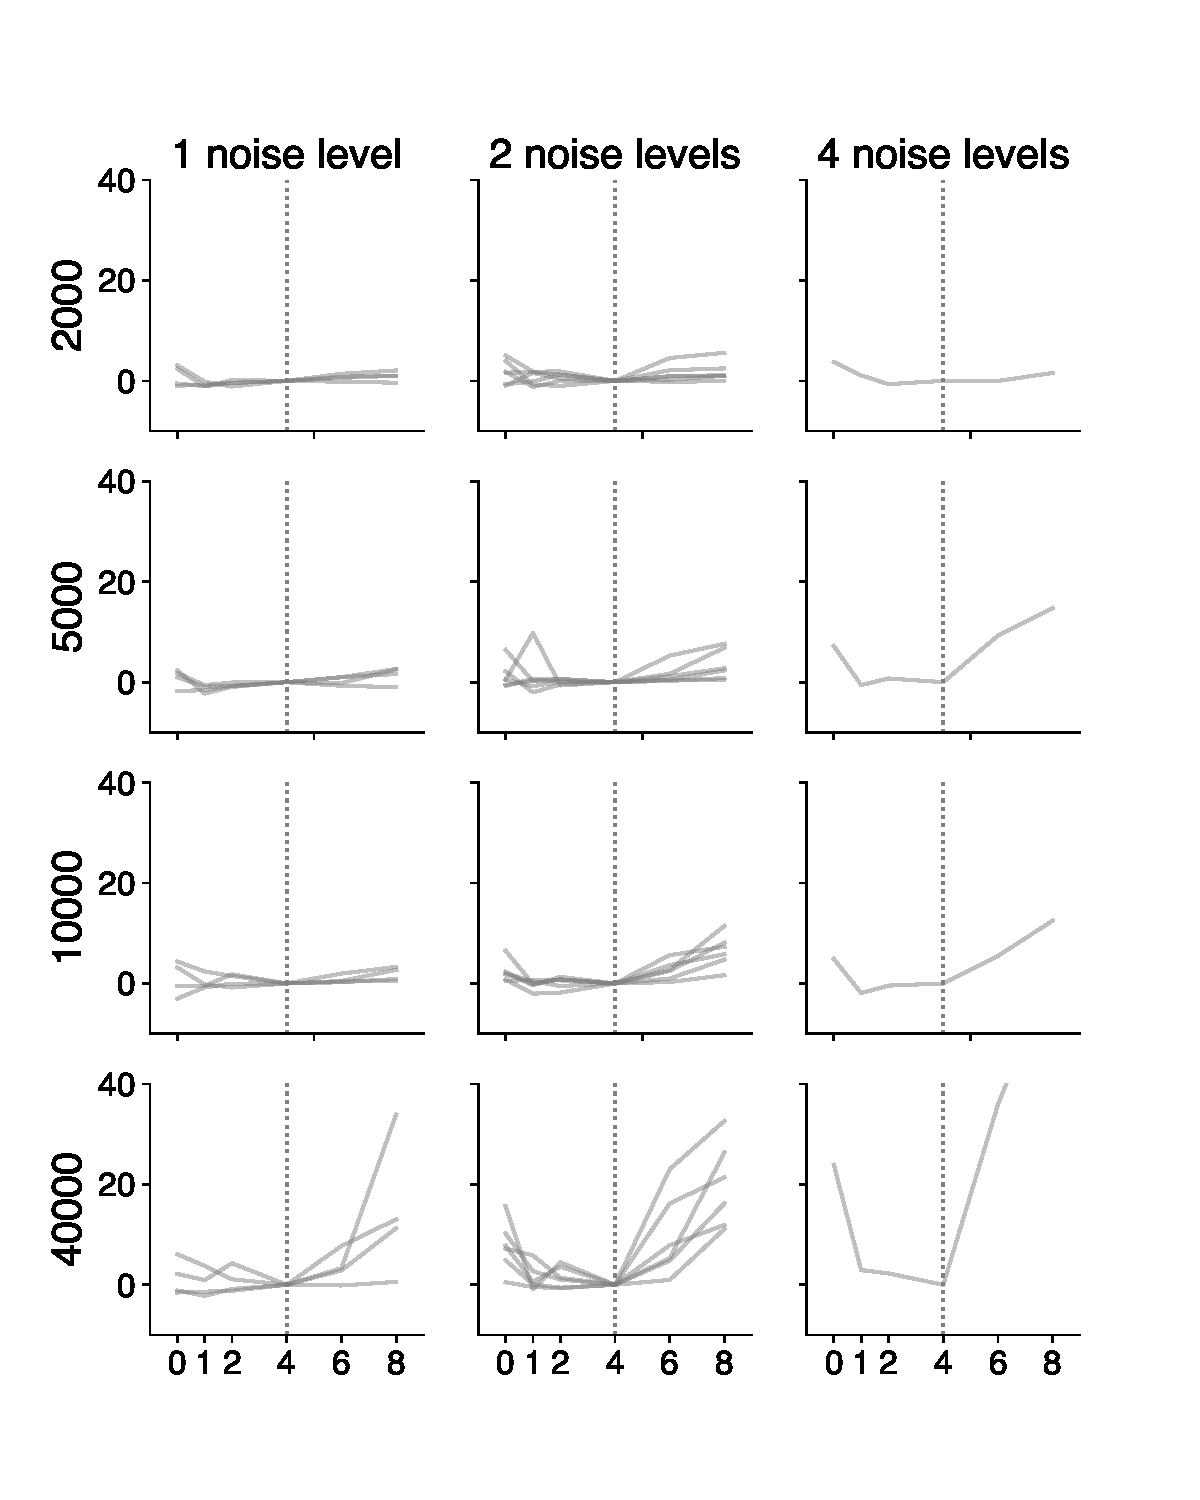
\includegraphics[width=1.1\linewidth]{figures/evaluateCrossValidationResults_Synthetic_Gardelle_VisualizeByNoiseCount_AndSize_ByP_Poster_Exculde1_Figure5.py_STEEPPERIODIC_STEEPPERIODIC_4.pdf}};

\node (U1) at (-7,2) {  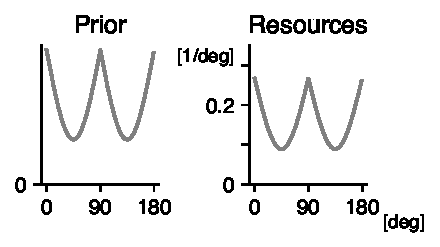
\includegraphics[width=0.7\textwidth]{figures/CounterfactualModel_VIZ_Components_Fig5.py_5_STEEPPERIODIC_STEEPPERIODIC_2_0_10.0_180.pdf}};
  \node [anchor=north] at (-12,4.5)    {\LARGE{a}};
  \node [anchor=north] at (-12,-0.5)    {\LARGE{b}};

\node[below=1cm of U1, xshift=0.15cm, yshift=-13.9cm, font=\fontsize{11pt}{13pt}\selectfont\sffamily] (E1) {exponent};
\node[below=1cm of U1, xshift=3.80cm, yshift=-13.9cm, font=\fontsize{11pt}{13pt}\selectfont\sffamily] (E2) {exponent};
\node[below=1cm of U1, xshift=-3.54cm, yshift=-13.9cm, font=\fontsize{11pt}{13pt}\selectfont\sffamily] (E3) {exponent};

%TODO fix color scale and color legend

 %  \includegraphics[width=0.8\linewidth]{../code/Synthetic/output/images/confusion-summary.pdf}

  %
  % ========================================================================
  % 1) ROW 1: Place the four heatmaps for N = 2,000
  % ========================================================================
  %
  % 1a) Put the first heatmap's top‐left corner at (0,0)
  \node (H11) [anchor=north west] at (0,-0.5)
    {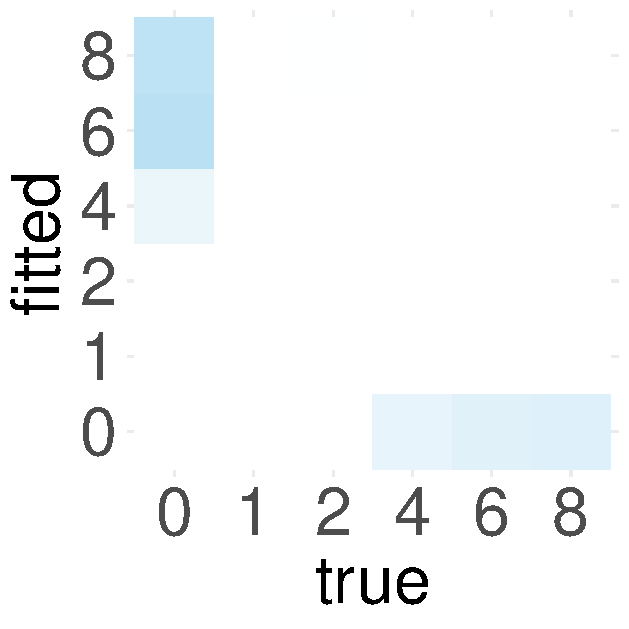
\includegraphics[width=0.29\textwidth]{../code/Synthetic/output/images/heatmap_dataSize_2000_noiseCount_1.pdf}};
  % 1b) Place the next three heatmaps to the right, each 2 mm apart
  \node (H12) [anchor=north west, right=2mm of H11] 
    {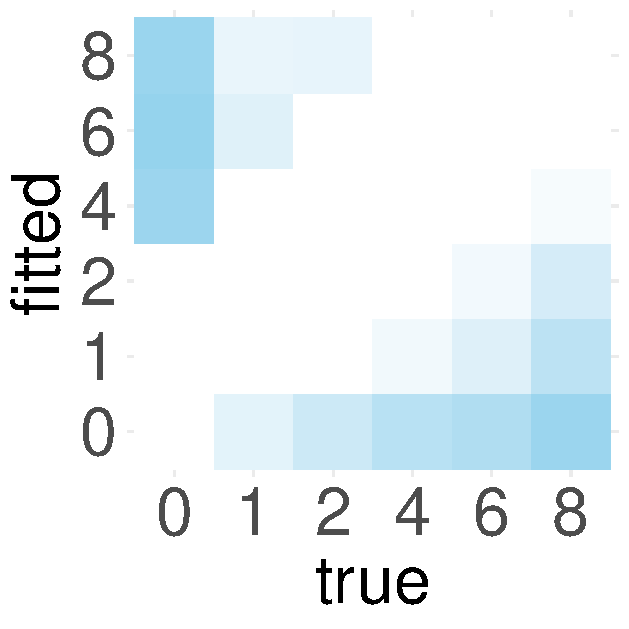
\includegraphics[width=0.29\textwidth]{../code/Synthetic/output/images/heatmap_dataSize_2000_noiseCount_2.pdf}};
  \node (H14) [anchor=north west, right=2mm of H12] 
    {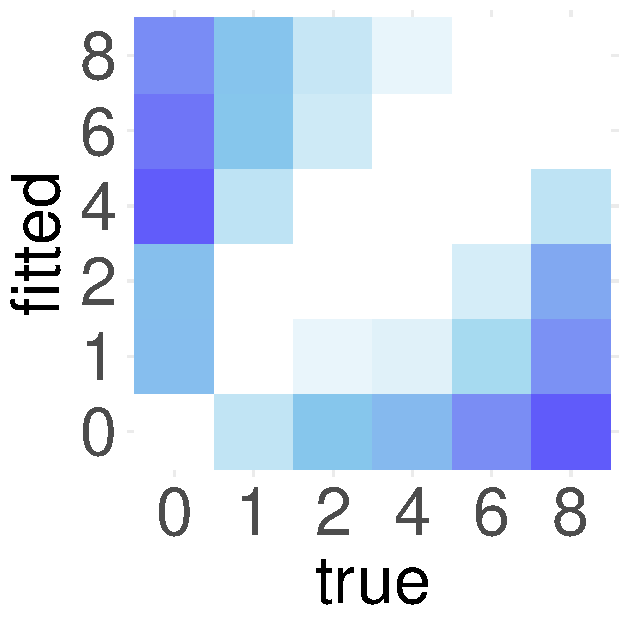
\includegraphics[width=0.29\textwidth]{../code/Synthetic/output/images/heatmap_dataSize_2000_noiseCount_4.pdf}};
  %\node (H14) [anchor=north west, right=2mm of H13] 
  %  {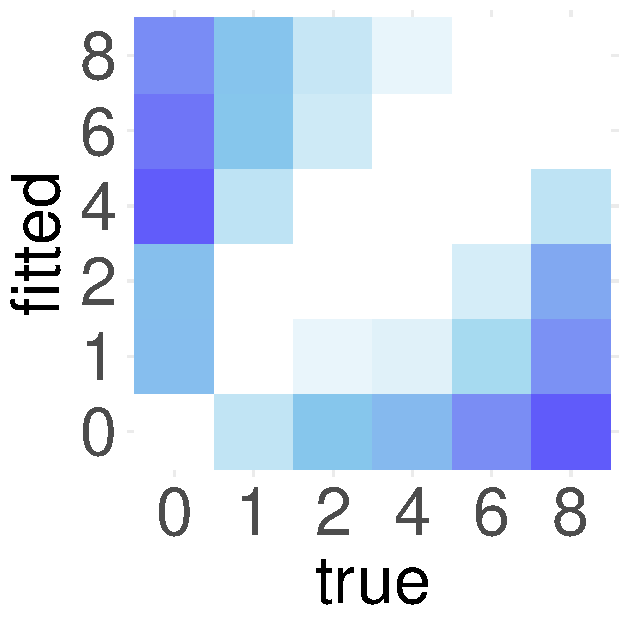
\includegraphics[width=0.23\textwidth]{../code/Synthetic/output/images/heatmap_dataSize_2000_noiseCount_4.pdf}};



  \node (SUM) [anchor=north] at (5.5,5)
    {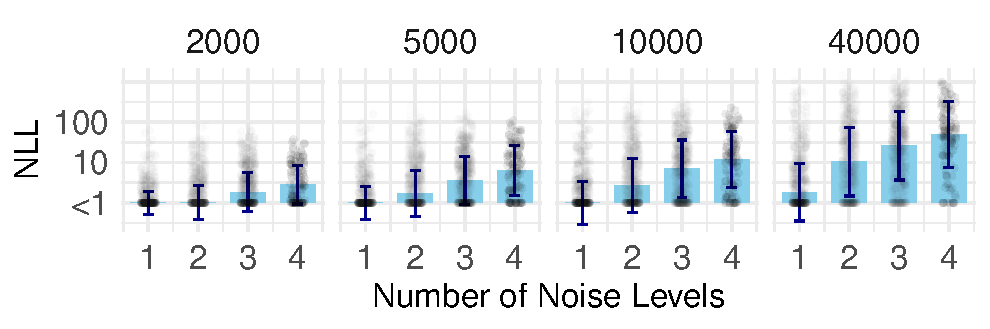
\includegraphics[width=0.99\textwidth]{../code/Synthetic/output/images/confusion‐summary‐with‐dots‐log‐sd.pdf}};
  \node [anchor=north] at ($(H11.north west)+(-0.5,50mm)$)    {\LARGE{c}};




  % 1c) Compute the midpoint between H11.north west and H14.north east
  \node[coordinate] (Row1TopCenter)
    at ($ (H11.north west)!0.5!(H14.north east) $) {};

  \node [anchor=north] at ($(H11.north west)+(-0.5,1cm)$)    {\LARGE{d}};



  % 1d) Place the “N=2,000 trials” label 2 mm above that midpoint
  \node (L1) [anchor=south, rotate=90,font=\fontsize{13pt}{15pt}\selectfont\sffamily] at ($(Row1TopCenter)+(-59mm,-15mm)$)    {2000};
  \node [anchor=south, rotate=90,font=\fontsize{13pt}{15pt}\selectfont\sffamily] at ($(Row1TopCenter)+(-59mm,-15mm-41mm)$)    {5000};
  \node [anchor=south, rotate=90,font=\fontsize{13pt}{15pt}\selectfont\sffamily] at ($(Row1TopCenter)+(-59mm,-15mm-2*41mm)$)    {10000};
  \node [anchor=south, rotate=90,font=\fontsize{13pt}{15pt}\selectfont\sffamily] at ($(Row1TopCenter)+(-59mm,-15mm-3*41mm)$)    {40000};

  %
  % ========================================================================
  % 2) ROW 2: Place the four heatmaps for N = 5,000, 12 mm below row 1
  % ========================================================================
  %
  % 2a) Anchor H21 so that its top‐left is 12 mm below H11’s bottom‐left
  \node (H21) [anchor=north west, below=4mm of H11.south west, xshift=1.85cm]
    {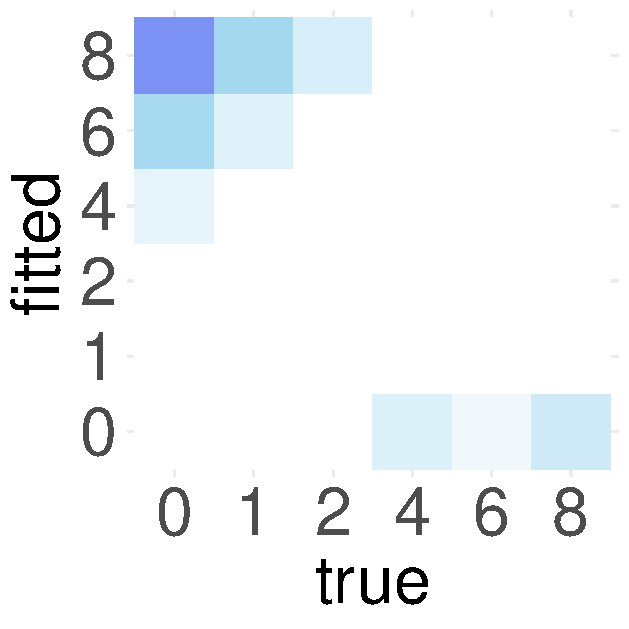
\includegraphics[width=0.29\textwidth]{../code/Synthetic/output/images/heatmap_dataSize_5000_noiseCount_1.pdf}};
  % 2b) Place the other three in row 2, 2 mm apart horizontally
  \node (H22) [anchor=north west, right=2mm of H21]
    {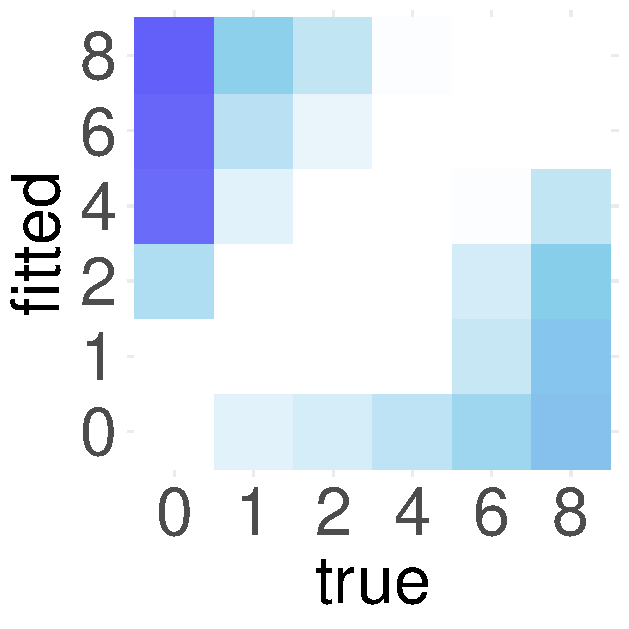
\includegraphics[width=0.29\textwidth]{../code/Synthetic/output/images/heatmap_dataSize_5000_noiseCount_2.pdf}};
  \node (H24) [anchor=north west, right=2mm of H22]
    {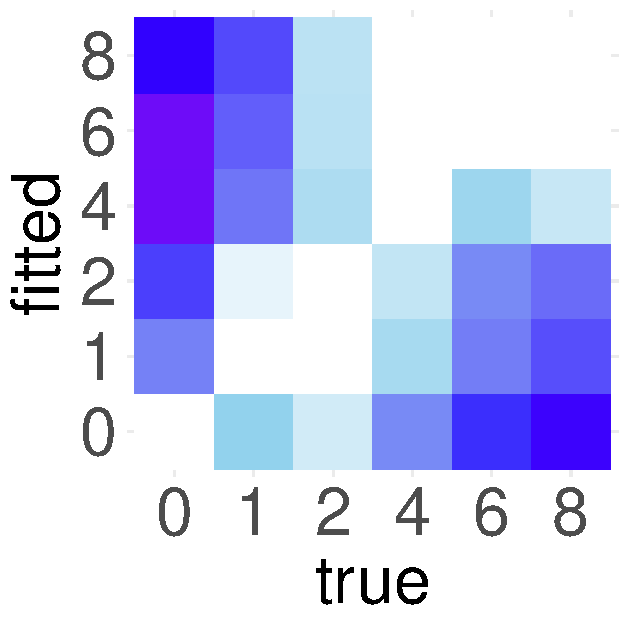
\includegraphics[width=0.29\textwidth]{../code/Synthetic/output/images/heatmap_dataSize_5000_noiseCount_4.pdf}};
  %\node (H24) [anchor=north west, right=2mm of H23]
  %  {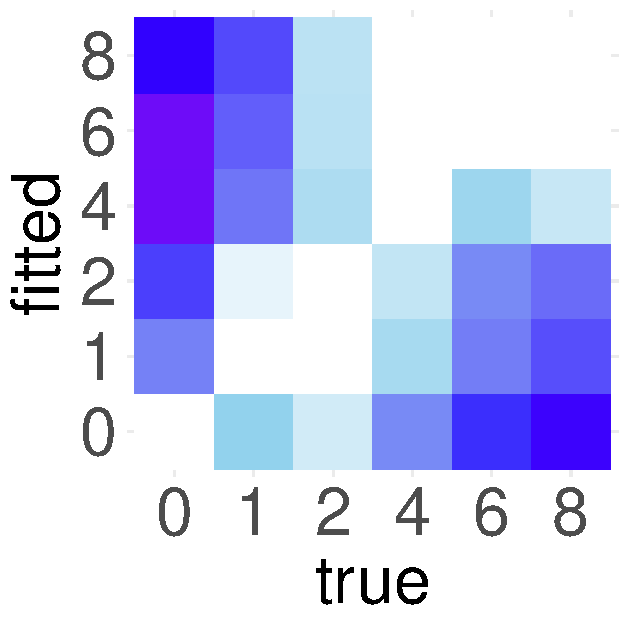
\includegraphics[width=0.23\textwidth]{../code/Synthetic/output/images/heatmap_dataSize_5000_noiseCount_4.pdf}};

  % 2c) Compute the midpoint above row 2’s four heatmaps
  \node[coordinate] (Row2TopCenter)
    at ($ (H21.north west)!0.5!(H24.north east) $) {};

  % 2d) Place the “N=5,000 trials” label 2 mm above that midpoint
  % \node (L2) [anchor=south] at ($(Row2TopCenter)+(0,-1mm)$)
  %   {\large\sffamily N=5{,}000 trials};

  %
  % ========================================================================
  % 3) ROW 3: Place the four heatmaps for N = 10,000, 12 mm below row 2
  % ========================================================================
  %
  \node (H31) [anchor=north west, below=4mm of H21.south west, xshift=1.85cm]
    {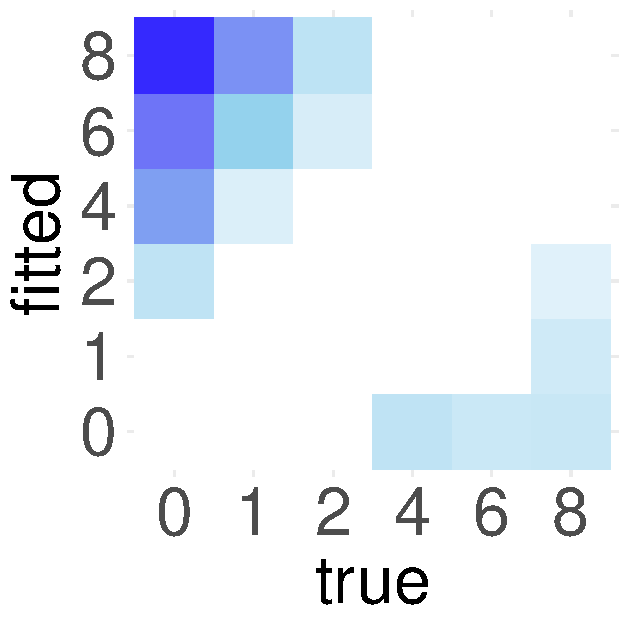
\includegraphics[width=0.29\textwidth]{../code/Synthetic/output/images/heatmap_dataSize_10000_noiseCount_1.pdf}};
  \node (H32) [anchor=north west, right=2mm of H31]
    {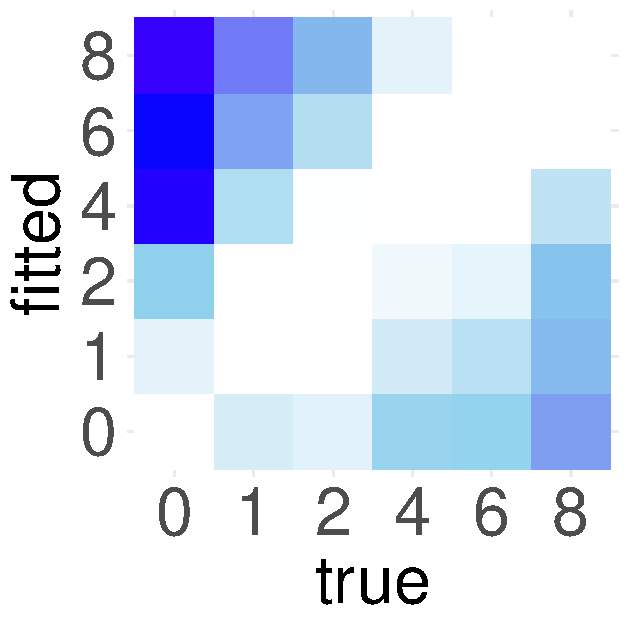
\includegraphics[width=0.29\textwidth]{../code/Synthetic/output/images/heatmap_dataSize_10000_noiseCount_2.pdf}};
  \node (H34) [anchor=north west, right=2mm of H32]
    {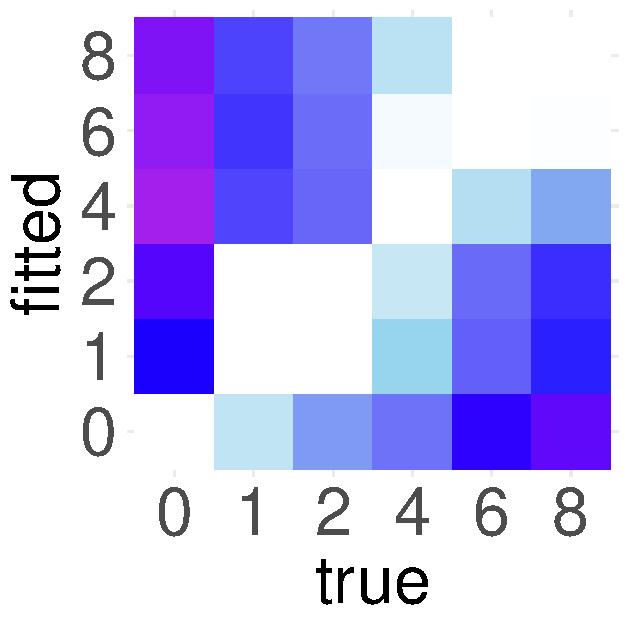
\includegraphics[width=0.29\textwidth]{../code/Synthetic/output/images/heatmap_dataSize_10000_noiseCount_4.pdf}};
%  \node (H34) [anchor=north west, right=2mm of H33]
 %   {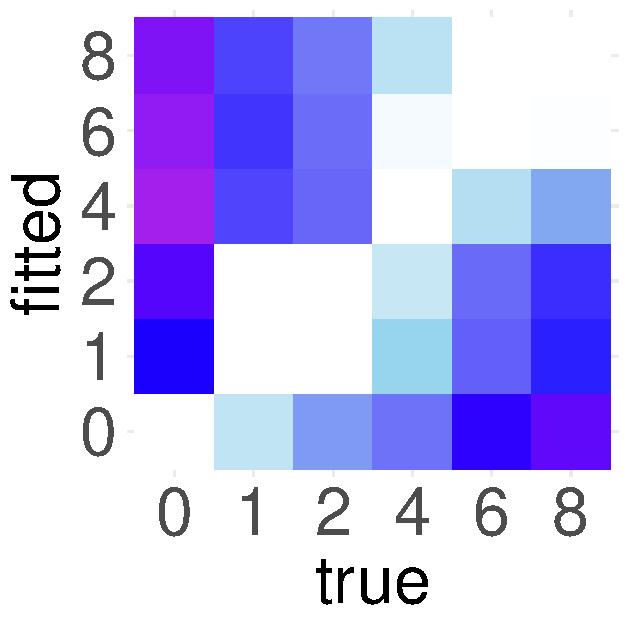
\includegraphics[width=0.23\textwidth]{../code/Synthetic/output/images/heatmap_dataSize_10000_noiseCount_4.pdf}};

  \node[coordinate] (Row3TopCenter)
    at ($ (H31.north west)!0.5!(H34.north east) $) {};
  % \node (L3) [anchor=south] at ($(Row3TopCenter)+(0,-1mm)$)
  %   {\large\sffamily N=10{,}000 trials};

  %
  % ========================================================================
  % 4) ROW 4: Place the four heatmaps for N = 40,000, 12 mm below row 3
  % ========================================================================
  %
  \node (H41) [anchor=north west, below=4mm of H31.south west, xshift=1.85cm]
    {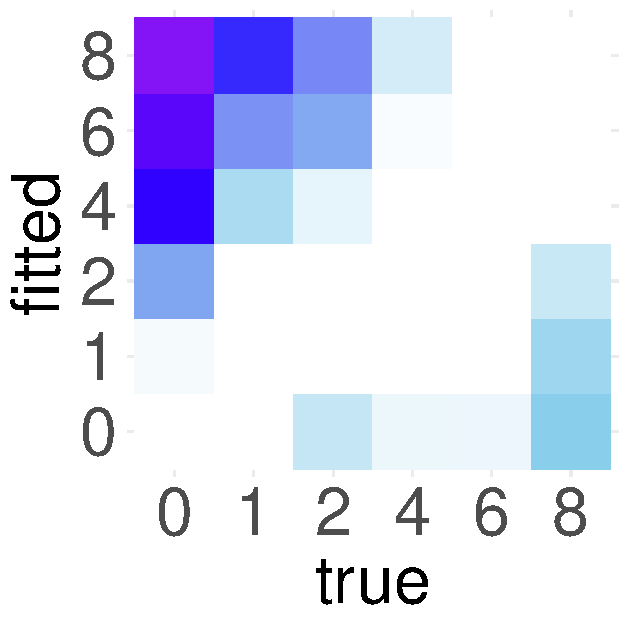
\includegraphics[width=0.29\textwidth]{../code/Synthetic/output/images/heatmap_dataSize_40000_noiseCount_1.pdf}};
  \node (H42) [anchor=north west, right=2mm of H41]
    {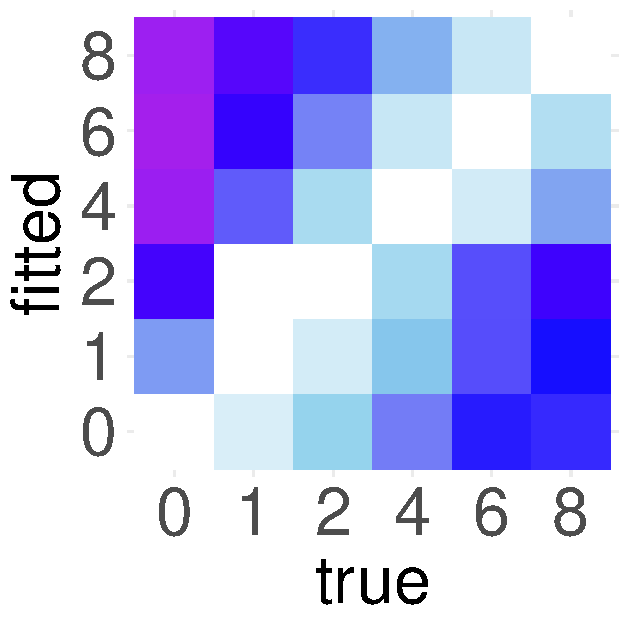
\includegraphics[width=0.29\textwidth]{../code/Synthetic/output/images/heatmap_dataSize_40000_noiseCount_2.pdf}};
  \node (H44) [anchor=north west, right=2mm of H42]
    {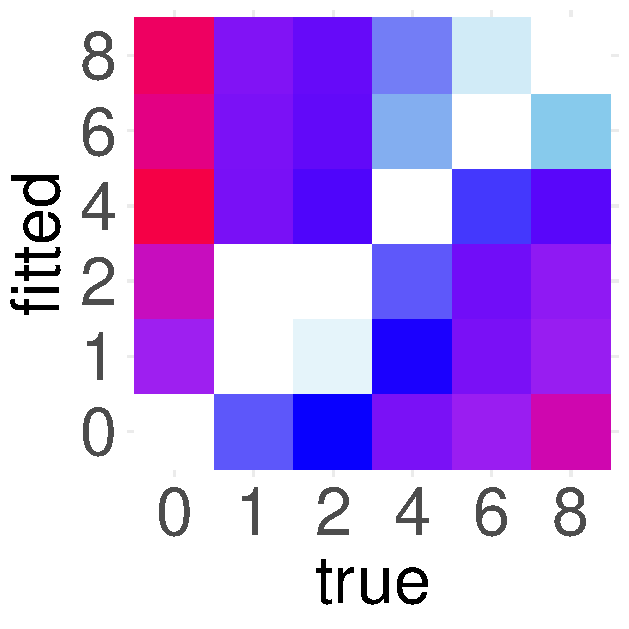
\includegraphics[width=0.29\textwidth]{../code/Synthetic/output/images/heatmap_dataSize_40000_noiseCount_4.pdf}};
%  \node (H44) [anchor=north west, right=2mm of H43]
 %   {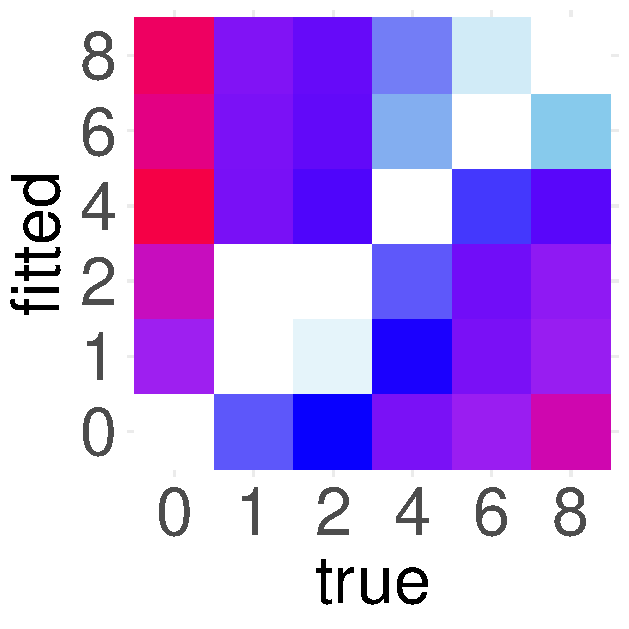
\includegraphics[width=0.23\textwidth]{../code/Synthetic/output/images/heatmap_dataSize_40000_noiseCount_4.pdf}};

  \node (H51) [anchor=north, above=2mm of H11.north, xshift=0.1cm]    {\Large{1 noise level}};
  \node (H52) [anchor=north, above=2mm of H12.north, xshift=0.1cm]    {\Large{2 noise levels}};
%  \node (H53) [anchor=north, above=2mm of H13.north, xshift=0.1cm]    {\Large{3 noise levels}};
  \node (H54) [anchor=north, above=2mm of H14.north, xshift=0.1cm]    {\Large{4 noise levels}};


  \node[coordinate] (Row4TopCenter)
    at ($ (H41.north west)!0.5!(H44.north east) $) {};
  % \node (L4) [anchor=south] at ($(Row4TopCenter)+(0,-1mm)$)
  %   {\large\sffamily N=40{,}000 trials};

  %
  % ========================================================================
  % 5) LEGEND: Centered below row 4’s heatmaps
  % ========================================================================
  %
  \node[coordinate] (Row4BotCenter)
    at ($ (H41.south west)!0.5!(H44.south east) $) {};
  \node (LEG) [anchor=north] at ($(Row4BotCenter)+(75mm,85mm)$)
    {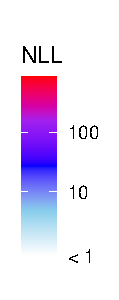
\includegraphics[width=0.2\textwidth]{../code/Synthetic/output/images/legend_only.pdf}};

  %
  % ========================================================================
  % 6) BOTTOM SUMMARY PLOT: Centered below the legend
  % ========================================================================
  %

\end{tikzpicture}
\end{document}

